\documentclass[aspectratio=43,hyperref={pdfpagelabels=false}]{beamer}	 	
\usepackage{lmodern}
\usepackage{abnt-alf}
\usepackage[brazil]{babel}
\usepackage{graphicx} \graphicspath{ {img/} } % Inclusão de gráficos
\usepackage[utf8]{inputenc}		% Codificacao do documento (conversão automática dos acentos)
\usepackage{multicol}
\usepackage{subfigure}
\usepackage{booktabs}

\usetheme{Berlin}
\usecolortheme{beaver}
\usefonttheme[onlymath]{serif}			% para fontes matemáticas
\definecolor{wine}{HTML}{8F0000}
\newcommand*\oldmacro{}%
\let\oldmacro\insertshorttitle%
\renewcommand*\insertshorttitle{%
  \oldmacro\hfill%
  \insertframenumber\,/\,\inserttotalframenumber}

\title[zorandir@gmail.com]{Diferença entre Templates de Autômatos Celulares Unidimensionais Binários}  
\author[ ]{Zorandir Soares Jr. \\zorandir@gmail.com} 
\institute[ ]{Universidade Presbiteriana Mackenzie\\
Programa de Pós-Graduação em Engenharia Elétrica e Computação \vskip 0.5cm
Orientador: Prof. Dr. Pedro Paulo Balbi de Oliveira
}
\date{\today} 

\begin{document}

\begin{frame}
    \titlepage
\end{frame}

\begin{frame}
% \begin{multicols}{2}
    \frametitle{Sumário}
    \tableofcontents
%\end{multicols}
\end{frame}




 
 \section[Objetivos]{Objetivos}
 \subsection*{Objetivos}
 \begin{frame}
     \frametitle{Objetivos}
     \begin{itemize}
           \item Apresentar a operação de diferença entre templates
           \item Apresentar a operação geradora de templates de exceção
           \item Apresentar exemplos da utilização dos templates no problema de paridade
     \end{itemize}
 \end{frame}
 
 




 \section{Autômatos Celulares}
 \subsection*{Autômatos Celulares}
 \begin{frame}
    \frametitle{Autômatos Celulares}

    \begin{figure}[h!]
        \centering
        
\includegraphics[width=0.6\textwidth]{fig_carpet.jpg}
        \caption{Tapetes expostos em uma exposição de arte realizada na ``Maison Salvan'', em Carjac, França, em junho de 2008. Eles foram criados com o simulador FiatLux CA.}
    \end{figure}

     % Autômatos Celulares (ACs) são idealizações matemáticas simples dos sistemas naturais. Eles consistem em um reticulado de campos discretos idênticos, onde cada campo pode assumir um conjunto finitos de, geralmente, valores inteiros. Os valores dos campos evoluem em tempo discreto de acordo com regras determinísticas que especificam o valor de cada campo de acordo com os campos das vizinhanças \cite{wolfram1994cellular}.
 \end{frame}

  



\begin{frame}
\frametitle{Famílias de autômatos celulares}
Uma família (ou espaço) de autômatos celulares é definida pelo raio $r$ e pelo número de estados $k$.

O tamanho de uma família é definido pela expressão abaixo:
\begin{equation}
k^{k^{2r+1}}
\label{eq:tamFamilia}
\end{equation}
\end{frame}

 \begin{frame}
     \frametitle{Propriedades Estáticas}
     \begin{itemize}
           \item Confinamento
           \item Simetria Interna Máxima
           \item Simetria Interna Arbitrária
           \item Totalidade e Semi-totalidade
           \item Conservabilidade da soma de estados
           \item Conservabilidade da soma modular de estados %(ou conservabilidade modular) %?
     \end{itemize}
 \end{frame}

\section{Templates}
\subsection*{Templates}
\begin{frame}
	\frametitle{Templates}
	
	\textit{Template} é uma generalização de tabelas de transições de ACs.
    \begin{figure}[h!]
        \centering
        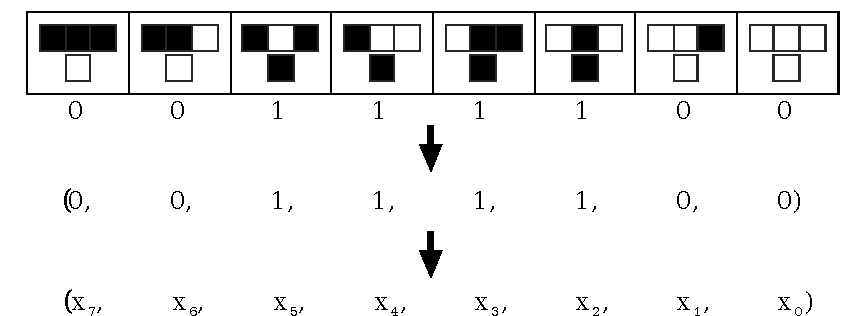
\includegraphics[width=0.6\textwidth]{fig_transitionTable.pdf}
        \caption{Exemplo de tabelas de transições}
    \end{figure}
\end{frame}

% \begin{frame}
%     \frametitle{Exemplo -  Template Base}
    
%     \begin{equation}
%     \begin{split}
%     (x_7,x_6,x_5,x_4,x_3,x_2,x_1,x_0)
%     \end{split}
%     \end{equation}
% \end{frame}

\begin{frame}
	\frametitle{Expansão}
	Expansão é o processo no qual se obtêm todas as tabelas de transição $R_k$ associadas a um template $T$.
  \begin{equation}
  E(T)=R_k
  \end{equation}
 \end{frame}

\begin{frame}
    \frametitle{Exemplo -  Expansão}
    
  \begin{table}[h!]
  \centering
  \caption{Processo de expansão do template $(1,1,1,1,1,x_0+x_1,x_1,x_0)$}
    \begin{tabular}{cccc}
      \toprule
    $i$ & $x_1$ & $x_0$ & tabela $k$-ária resultante \\
      \midrule
    0 & 0 & 0 & (1,1,1,1,1,0,0,0) \\
    1 & 0 & 1 & (1,1,1,1,1,1,0,1) \\
    2 & 1 & 0 & (1,1,1,1,1,1,1,0) \\
    3 & 1 & 1 & (1,1,1,1,1,2,1,1) \\
      \bottomrule
      \end{tabular}
  \label{tab:invalideExpansion}
  \end{table}
\end{frame}

\begin{frame}
	\frametitle{Intersecção}
	\begin{equation}
	I(T_1,T_2)=T_3 \Leftrightarrow E(T_3) = E(T_1) \cap E(T_2)
	\end{equation}

    \begin{figure}[h!]
      \centering
      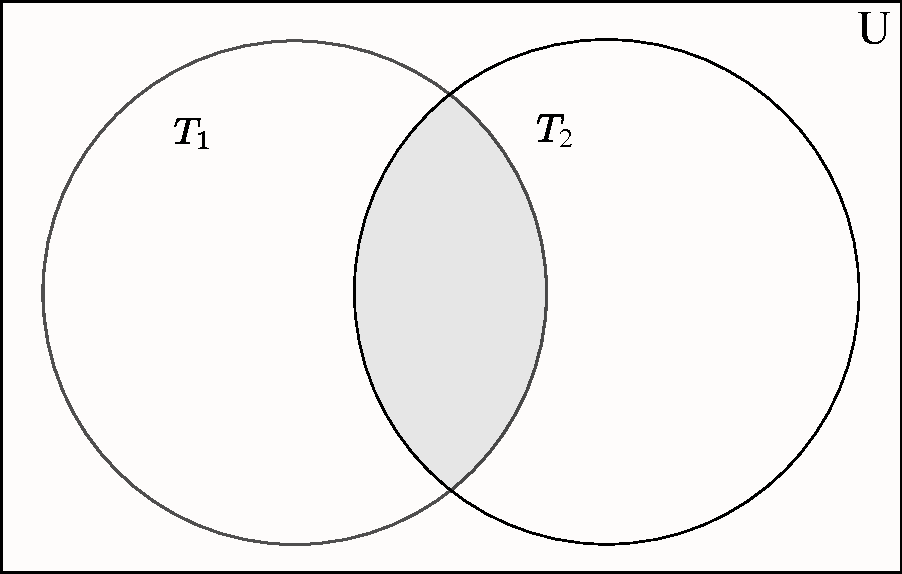
\includegraphics[width=.4\textwidth]{fig_intersection.pdf}
      \caption{Os círculos $T_1$ e $T_2$ são templates que representam dois conjuntos de regras. Em cinza, $T_3$ é o template que representa o conjunto de regras de intersecção entre $T_1$ e $T_2$.}
      \label{fig:intersection}
    \end{figure}        
    % Intersecção é o processo no qual se obtêm um template que represente o conjunto $R_k$ após se receber dois templates definidos para o mesmo espaço. A operação de intersecção também foi implementada por \cite{daCosta2014} e foi descrita em maior detalhes da seguinte maneira:

 \end{frame}

 \begin{frame}
    \frametitle{Geradoras de Templates e Número de Estados}
    \vspace{-0.8cm}
    \begin{table}[]
    \centering
    \caption{Compatibilidade entre algoritmos geradores de templates e número de estados }
    \vspace{-0.8cm}
    \label{my-label}
    \resizebox{\textwidth}{!}{
    \vspace{0cm}
    \begin{tabular}{|l|l|l|}
    \hline
                                               & \multicolumn{2}{c|}{Número de Estados} \\ \hline
    \textbf{Algoritmos Geradores de Templates} & $k=2$                              & $k\textgreater2$                          \\ \hline
    Totalidade e Semi-Totalidade               &  •                                 & •                                         \\ \hline
    Confinamento                               &  •                                 & •                                         \\ \hline
    Color Blind                                &  •                                 & •\footnote{Template Modular}              \\ \hline
    Simetria Máxima                            &  •                                 & •                                         \\ \hline
    Simetria Arbitrária                        &  •                                 &                                           \\ \hline
    Conservabilidade da soma de estados                &  •                                 & •                                         \\ \hline
    Conservabilidade da soma modular de estados                &  •\footnotemark[\value{footnote}]  &                                           \\ \hline
    \hline
    \end{tabular}
    }
\end{table}
\end{frame} 


 \begin{frame}
    \frametitle{Geradoras de Templates e Pós-processamentoj}
    \vspace{-0.8cm}
\begin{table}[h!]
\centering
\caption{Pós-processamento necessário por templates}
    \vspace{-0.8cm}
    \resizebox{\textwidth}{!}{%
  \begin{tabular}{ll}
    \toprule
  Template & Pós-processamento \\
    \midrule
  Template de regras confinadas         & Filtrar regras com restrições inválidas \\
  Template de conservabilidade de estados   & Filtrar regras inválidas            \\
  Template de conservabilidade de paridade  & Aplicar $mod$ $2$ e filtrar regras inválidas  \\
  Template de totalidade e semi-totalidade  & Nenhum pós-processamento necessário         \\
  Templates de simetria           & Nenhum pós-processamento necessário         \\
    \bottomrule
  \end{tabular}
  }
\label{tab:posProcessamento}
\end{table}
\end{frame} 


 \section{Diferença entre Templates}
 \subsection*{Diferença entre Templates}
 \begin{frame}
     \frametitle{Diferença entre Templates}
     \begin{itemize}
           \item Templates de exceção
           \item Diferença entre Templates
     \end{itemize}
 \end{frame}

 \begin{frame}
     \frametitle{Templates de exceção}

      A operação geradora de templates de exceção $X$ gera um conjunto $C_e$ com todos os templates de exceção do template $T_o$ passado como parâmetro. A operação que gera o conjunto templates de exceção de um template pode ser descrita em mais detalhes da seguinte maneira:
      \begin{equation}
      \begin{split}
      X(T_o)= C_e \\
      C_e = \{T_1,T_2,\dots, T_n\}\\
      \end{split}
      \end{equation}     
 \end{frame}

 \begin{frame}
    \frametitle{Exemplo - Templates de exceção}
    
    \\Considere o template:
    $T_{o} = (1, x_6, x_5, 1 - x_1 - x_2, 2 - x_1 - x_2, x_2, x_1, 0)$. 

    O primeiro passo do algoritmo é encontrar um conjunto com as posições que não apresentem apenas constantes ou variáveis livres, obtendo-se assim $\{\{1 - x_1 - x_2\}, \{2 - x_1 - x_2\}\}$.
 \end{frame}
 \begin{frame}
     \frametitle{Templates de exceção}
    \begin{columns}
        \begin{column}{5cm}
          \begin{table}[h!]
          \centering
          \caption{Expansão do campo 1 - x_1 - x_2.}
            \begin{tabular}{ccc}
              \toprule
            $x_2$ & $x_1$ & Expansão do campo \\
              \midrule
            0 & 0 & 1 - x_1 - x_2 = 1 \\
            0 & 1 & 1 - x_1 - x_2 = 0 \\
            1 & 0 & 1 - x_1 - x_2 = 0 \\
            1 & 1 & 1 - x_1 - x_2 = -1  \\
              \bottomrule
            \end{tabular}
          \label{tab:exceptionProcessA}
          \end{table} 
        
        \end{column}
        \begin{column}{5cm}

          \begin{table}[h!]
          \centering
          \caption{Expansão do campo 2 - x_1 - x_2.}
            \begin{tabular}{ccc}
              \toprule
            $x_2$ & $x_1$ & Expansão do campo \\
              \midrule
            0 & 0 & 2 - x_1 - x_2 = 2 \\
            0 & 1 & 2 - x_1 - x_2 = 1 \\
            1 & 0 & 2 - x_1 - x_2 = 1 \\
            1 & 1 & 2 - x_1 - x_2 = 0 \\
              \bottomrule
            \end{tabular}
          \label{tab:exceptionProcessB}
          \end{table}

        \end{column}
\end{columns}
 \end{frame}
 \begin{frame}
     \frametitle{Templates de exceção}
Para finalizar a operação, o algoritmo seleciona as substituições que geram valores inválidos, e aplicam ela ao template base, gerando assim o conjunto de templates $C_e$, mostrado na  Eq. \ref{eq:exceptionsTemplates2}.

\begin{equation}
C_e = \{(x_7, x_6, x_5, x_4, x_3, 1, 1, x_0),(x_7, x_6, x_5, x_4, x_3, 0, 0, x_0)\}
\label{eq:exceptionsTemplates2}
\end{equation}
 \end{frame}

  \begin{frame}
    \frametitle{Operação de Diferença entre Templates Binários}

    A operação de diferença entre templates binários $D_i$ é responsável por obter um conjunto $C_{di}$ com $n$ templates, os quais, quando expandidos (via a operação de expansão $E$), apresentam apenas as regras geradas pela expansão do template $T_m$ que não estejam também presentes na expansão do template de intersecção entre $T_s$ e $T_m$, chamado aqui de $T_i$.
    \begin{equation}
    \begin{split}
    D_i(T_m,T_s)= C_{di} \Leftrightarrow E(C_{di}) = E(T_m) \setminus E(T_i) \\
    T_i = I(T_m,T_s)\\
    C_{di} = \{T_1,T_2,\dots, T_n\}\\
    \end{split}
    \end{equation}
 \end{frame}


  \begin{frame}
    \frametitle{Operação de Diferença entre Templates Binários}
    A Figura \ref{fig:complement} ilustra essa operação, onde os templates $T_m$ e $T_s$ passados como parâmetro para a operação de diferença estão representado pelos dois círculos, e o conjunto $C_{di}$ retornado pela função está representado pela área em cinza na imagem.
    \begin{figure}[h!]
      \centering
      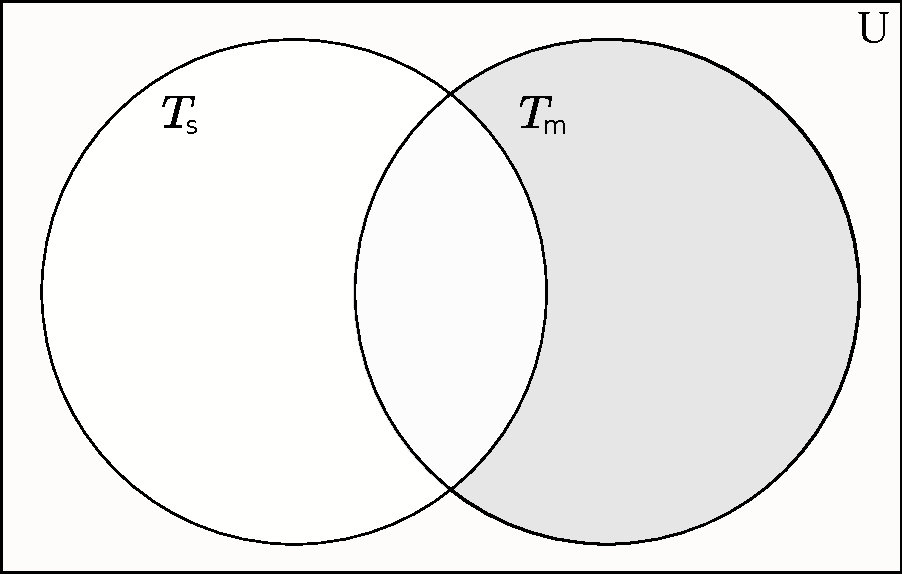
\includegraphics[width=.4\textwidth]{fig_complement2.pdf}
      \caption{Os círculos $T_m$ e $T_s$ são os templates que representam dois conjuntos de regras. Em cinza, $C_{di}$ é o conjunto de templates que representam o conjunto de regras retornado pela operação de diferença.}
      \label{fig:complement}
    \end{figure}
 \end{frame}

 \begin{frame}
    \frametitle{Exemplo - Operação de Diferença entre Templates}
    Considere
    \begin{equation}
    \begin{split}
    T_m = (x_7, x_6, x_5, x_4, x_3, x_1, x_1, x_0) \\
    T_s = (x_7, x_6, x_3 + x_1, 1 - x_1, x_3, x_1, x_1, 0)\\
    T_i = I(T_m,T_s) = (x_7, x_6, x_3 + x_1, 1 - x_1, x_3, x_1, x_1, 0)\\
    \end{split}
    \end{equation}
 \end{frame}

 \begin{frame}
    \frametitle{Exemplo - Operação de Diferença entre Templates}
    \begin{columns}
        \begin{column}{5cm}
    \begin{equation}
    \left\{\begin{matrix}
    x_7 & = & x_7 \\ 
    x_6 & = & x_6 \\ 
    x_5 & = & x_3 + x_1 \\ 
    x_4 & = & 1 - x_1 \\ 
    x_3 & = & x_3 \\ 
    x_1 & = & x_1 \\ 
    x_1 & = & x_1 \\ 
    x_0 & = & 0
    \end{matrix}\right.
    \end{equation}

    \end{column}

    \begin{column}{5cm}
    \begin{equation}\\
    x_7 = x_7 \wedge  
    x_6 = x_6 \wedge  \\
    x_5 = x_3 + x_1 \wedge  
    x_4 =   1 - x_1 \wedge  \\
    x_3 = x_3 \wedge  
    x_1 = x_1 \wedge  \\
    x_1 = x_1 \wedge  
    x_0 = 0
    \end{equation}

    \begin{equation}\\
    x_5 = x_3 + x_1 \\
    \vee x_4 = 1 - x_1 \\
    \vee x_0 = 0
    \label{eq:logicalComplement1}
    \end{equation}
    \end{column}
\end{columns}
\end{frame}

\begin{frame}
    \frametitle{Exemplo - Operação de Diferença entre Templates}

    \begin{equation}
    x_5 = 1 - (x_3 + x_1) \vee x_4 = 1 - (1 - x_1) \vee x_0 = 1 - 0
    \label{eq:logicalComplement2}
    \end{equation}

    \begin{equation}
    S = \{\{x_0 \to 1\}, \{x_4 \to x_1\}, \{x_5 \to 1 - x_1 - x_3\}\}
    \label{eq:logicalComplement3}
    \end{equation}

    \begin{equation}
    \begin{split}
    C_{di} = \{\\(x_7, x_6, x_5, x_4, x_3, x_1, x_1, 1), \\(x_7, x_6, x_5, x_1, x_3, x_1, x_1, x_0), \\(x_7, x_6, 1 - x_1 - x_3, x_4, x_3, x_1, x_1, x_0)\}
    \end{split}
    \label{eq:logicalComplement3}
    \end{equation}

\end{frame}

 \section{Discussões e Testes}
 \subsection*{Discussões e Testes}
 \begin{frame}
     \frametitle{Discussões e Testes}
     \begin{itemize}
           \item Aplicação no Problema de Paridade
           \item Metodologia de testes
     \end{itemize}
 \end{frame}

\begin{frame}
    \frametitle{Problema de Paridade}
    \begin{figure}[h!]
        \centering
        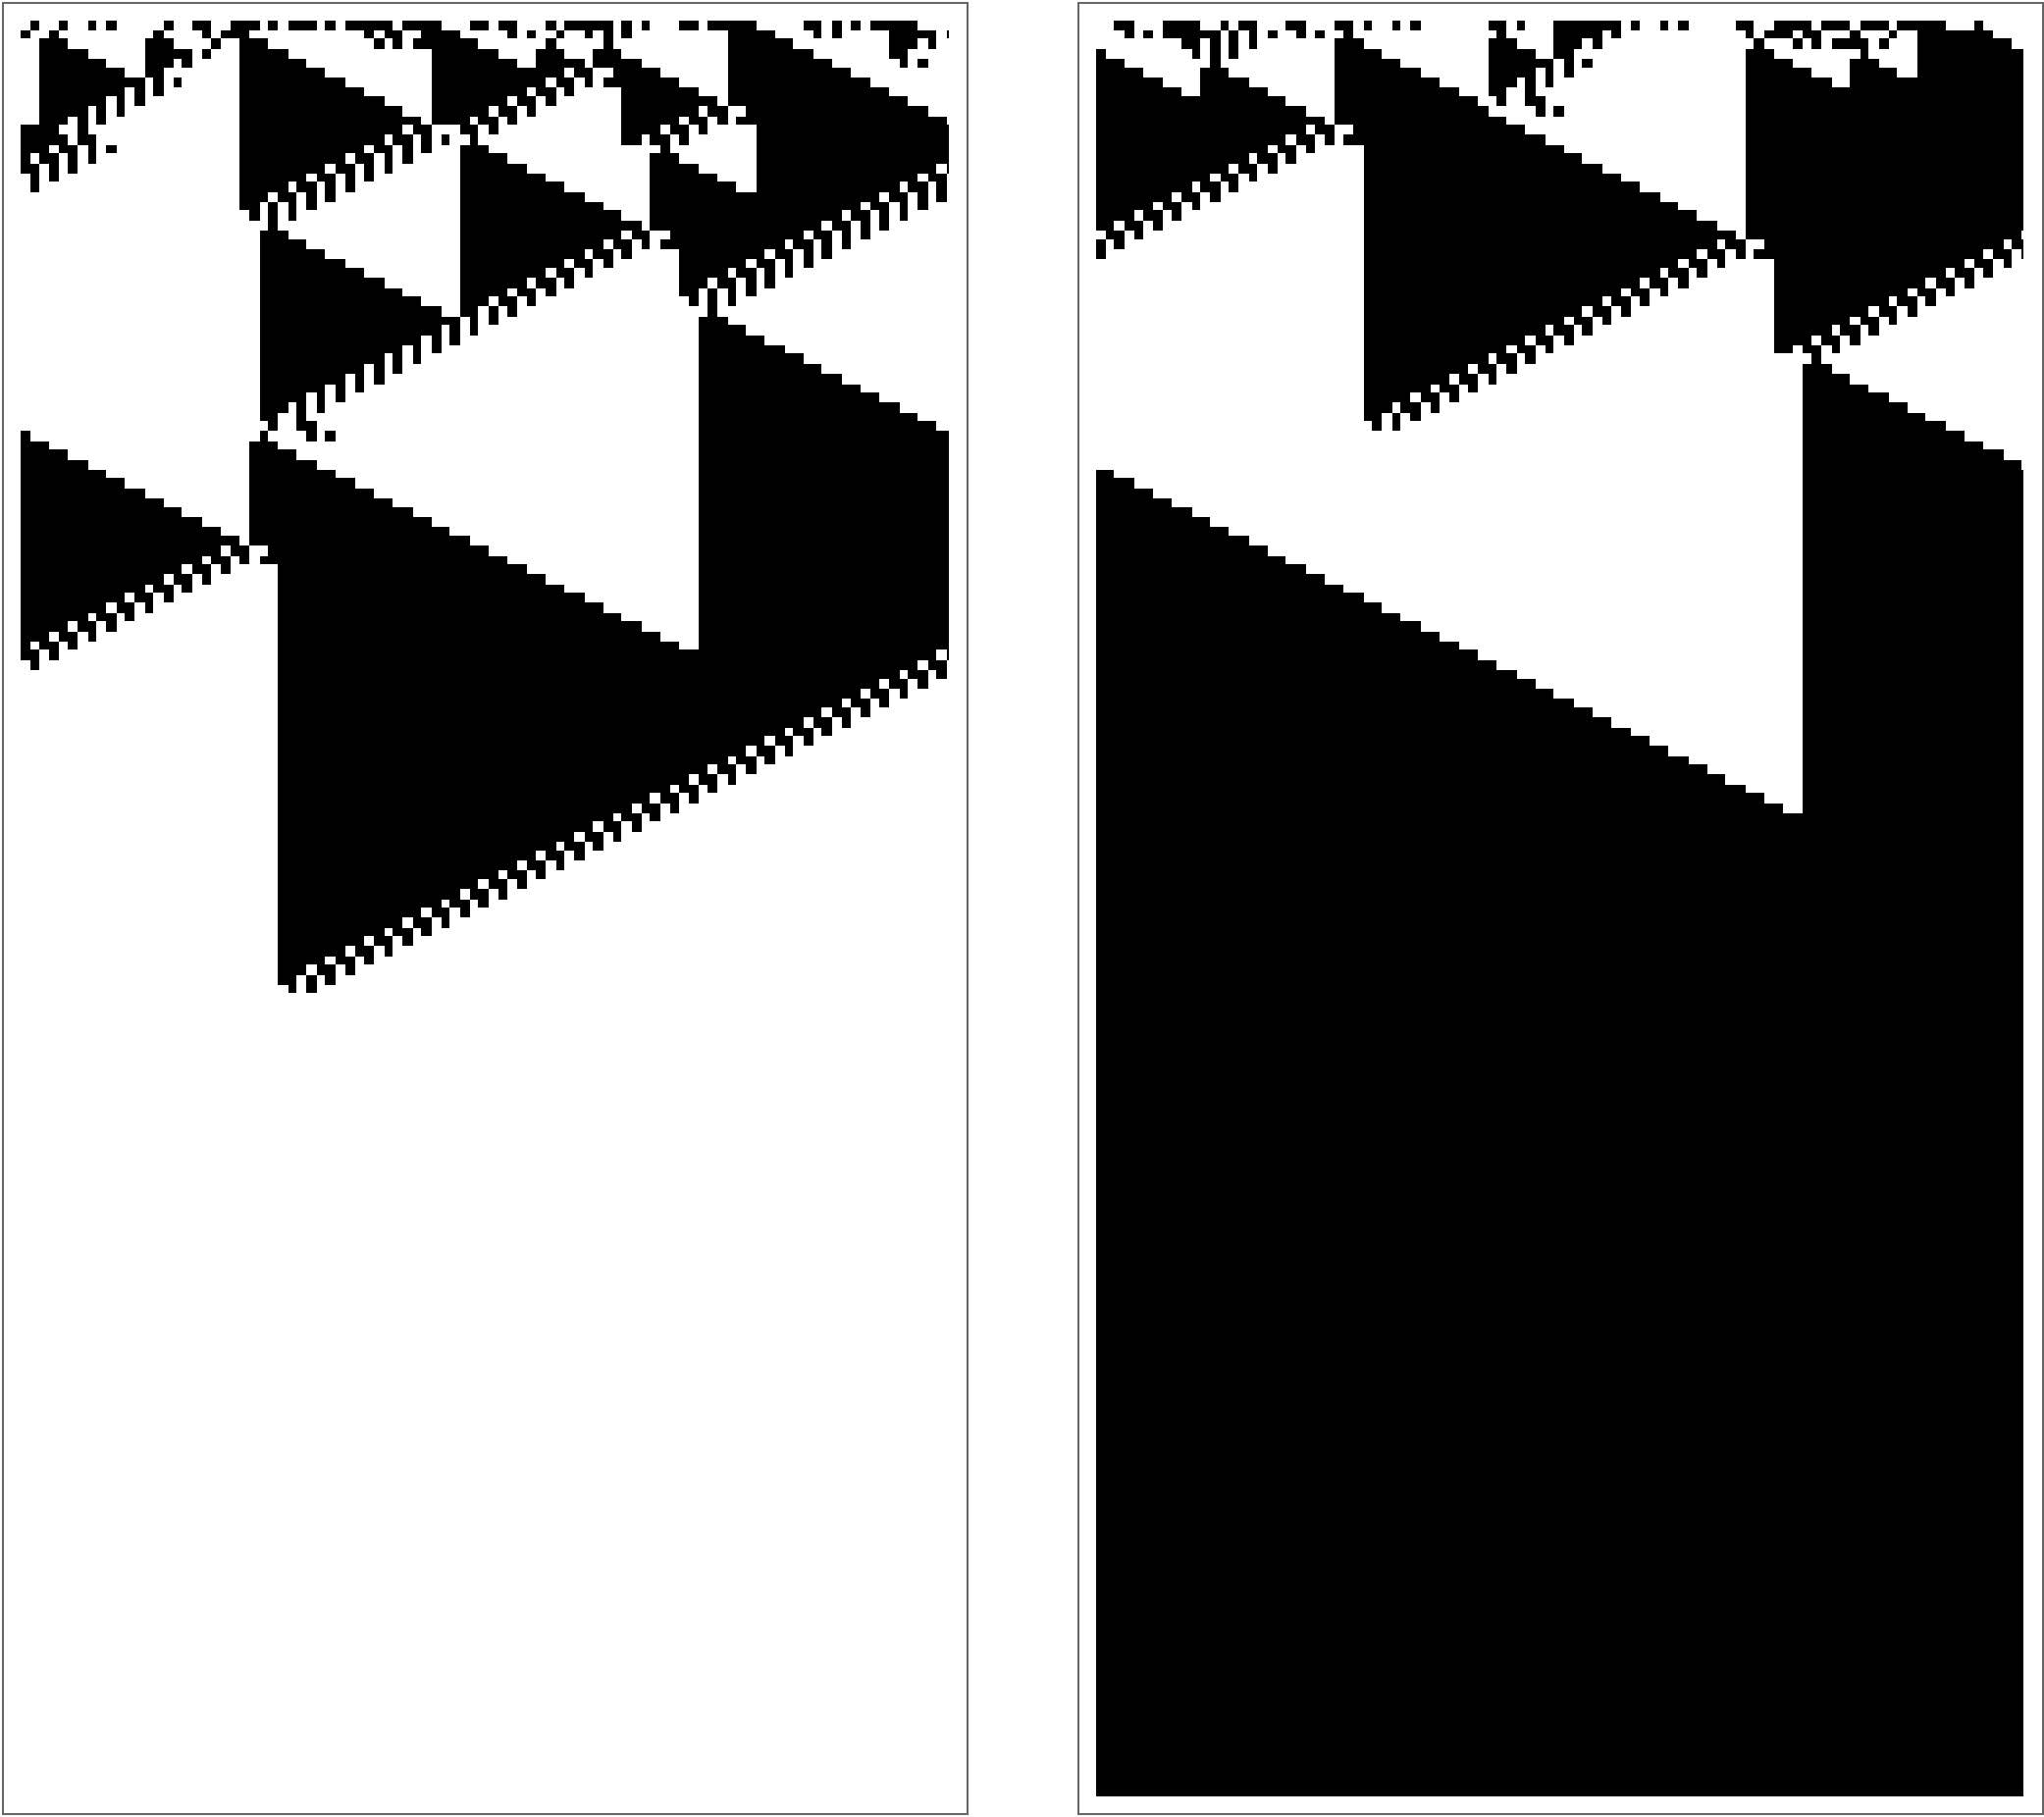
\includegraphics[width=0.5\textwidth]{fig_parityRule.pdf}
        \caption{Exemplo de regra de paridade. A imagem a esquerda contém em sua entrada um número par de 1s. A da direita contém um número ímpar.}
    \end{figure}
\end{frame}

\begin{frame}
    \frametitle{Problema de Paridade}
    \begin{equation}
    T_{paridade} = (T_{conservaparidade} \cap T_{confinado}) \cap \bar{T}_{conservaestados}
    % T_{paridade} = T_{conservaparidade} \cap \bar{T}_{conservaestados}
    \label{eq:operationsTemplateParidade}
    \end{equation}

    \begin{alertblock}{A regra que solucione o problema de paridade:}
        \vspace{-0.4cm}    
        \begin{itemize}
          \item deve ser \textbf{confinada}
          \item deve \textbf{conservar a paridade}
          \item não deve \textbf{number conserving}
        \end{itemize}
    \end{alertblock}
\end{frame}

\begin{frame}
    \frametitle{Problema de Paridade}

    Tamanho do espaço:
    \begin{equation}
    2^{2^{2\times3+1}}=3,4 \times 10^{38}
    \end{equation}

    Número máximo de regras conservativas de paridade:
    \begin{equation}
    2^{63} \approx  9.2\times 10^{18}
    \end{equation}
\end{frame}

\begin{frame}
    \frametitle{Testes}
    \vspace{-0.8cm}
    \begin{table}[h!]
    \centering
    \caption{Propriedades estáticas utilizadas para o teste da operação de diferença em cada raio}
    \vspace{-0.8cm}
    \resizebox{\textwidth}{!}{%
    \begin{tabular}{l|lllll|}
    \cline{2-6}
    & \multicolumn{5}{c|}{Template minuendo ($T_m$)} \\ \cline{1-1}
    \multicolumn{1}{|l|}{Template subtraendo ($T_s$)}                  
    & totalidade
    & semi-totalidade
    & \begin{tabular}[c]{@{}l@{}}conservabilidade\\ de estados\end{tabular} 
    & \begin{tabular}[c]{@{}l@{}}invariância à\\ troca de cor\end{tabular}  
    & confinamento 
    \\ \cline{2-6} 

    \multicolumn{1}{|l|}{totalidade}                  & Raio 1, 2 e 3& Raio 1, 2 e 3  & Raio 1 e 2& Raio 1 e 2& Raio 1  \\
    \multicolumn{1}{|l|}{semi-totalidade}             & Raio 1, 2 e 3& Raio 1, 2 e 3  & Raio 1 e 2& Raio 1 e 2& Raio 1  \\
    \multicolumn{1}{|l|}{conservabilidade de estados} & Raio 1 e 2   & Raio 1 e 2   & Raio 1 e 2& Raio 1 e 2& Raio 1  \\
    \multicolumn{1}{|l|}{invariância  à troca de cor} & Raio 1 e 2   & Raio 1 e 2   & Raio 1 e 2& Raio 1 e 2& Raio 1  \\
    \multicolumn{1}{|l|}{confinamento}                & Raio 1     & Raio 1     & Raio 1  & Raio 1  & Raio 1  \\ \hline
    \bottomrule
    \end{tabular}%
    }
    \label{tab:differenceTests}
    \end{table}
\end{frame}

% \section{Referências}
%  \begin{frame}%[allowframebreaks]
%      \frametitle{Referências}
%      \bibliography{bibliografia}
%  \end{frame}

\section*{}
\begin{frame}[t]
     \frametitle{Agradecimentos}
\vspace{1cm}
\center
     À Capes, CNPq, MackPesquisa e ao Laboratório de Computação Natural (LCoN).
\end{frame}
\end{document}
